\documentclass{article}

\usepackage[T1]{fontenc}
\usepackage[utf8]{inputenc}
\usepackage[french]{babel}
\usepackage{lmodern}
\usepackage[margin=1in]{geometry}
\usepackage{setspace}
\onehalfspacing
\setlength{\parindent}{0pt}
\setlength{\parskip}{0.45em}
\emergencystretch=2em

\usepackage{graphicx}
\graphicspath{{../}}
\usepackage{float}
\usepackage{caption}
\usepackage{tabularx}
\usepackage{booktabs}
\usepackage{array}
\usepackage{hyperref}
\hypersetup{pdfborder={0 0 0}}

\captionsetup{font=small,labelfont=bf}
\renewcommand{\thesection}{\arabic{section}.}
\renewcommand{\thesubsection}{\arabic{section}.\arabic{subsection}.}
\newcolumntype{Y}{>{\raggedright\arraybackslash}X}

\begin{document}

\hypersetup{pageanchor=false}
\begin{titlepage}
  \centering
  \vspace*{0.8cm}

  {\Large POLYPBASE\\[0.35cm]}
  \rule{\textwidth}{0.9pt}\\[0.5cm]
  {\Large \textbf{Mémoire technique sur la construction d’une webapp de suivi des polypes de méduses}}\\[0.35cm]
  {\large Aquarium de Paris}\\[0.4cm]
  \rule{\textwidth}{0.9pt}\\[1cm]

  \large
  Réalisé par\\[0.15cm]
  Anthony COMBES-AGUÉRA,\\
  Ayoub AKKOUH,\\
  et Clément ROMANET\\[0.55cm]

  \rule{0.5\textwidth}{0.9pt}\\[0.35cm]

  Encadré par\\[0.15cm]
  Anaïs COURTET\\
  et Étienne BOURGOUIN\\[0.55cm]

  \rule{0.5\textwidth}{0.9pt}\\[0.35cm]

  {\large Version de travail}\\[0.2cm]
  {\large 30 mai 2026}\\[1cm]

  \vfill
  {\footnotesize Année universitaire 2025-2026}
\end{titlepage}

\newpage
\thispagestyle{empty}
\vspace*{3cm}
\begin{center}
{\Large \textbf{Remerciements}}
\end{center}

\vspace{1cm}
Nous tenons à remercier Anaïs Courtet et Étienne Bourgouin pour leur accueil au sein de l’Aquarium de Paris et pour le temps qu’ils nous ont accordé depuis le début du stage. Leur disponibilité, leurs explications et leurs retours nous ont permis de mieux comprendre le fonctionnement du service des méduses et les besoins réels derrière Polypbase.

Nous les remercions aussi pour leur sympathie et pour la visite guidée de l’Aquarium. Cette découverte du lieu, des espaces ouverts au public et des coulisses nous a aidés à mieux situer notre travail. Polypbase accompagne un travail quotidien en laboratoire, dans un environnement vivant, précis et déjà très organisé.

Nous remercions également Madame Sophie Lebre, qui nous a transmis cette offre de stage. Son partage nous a permis de rejoindre un projet concret, utile et directement lié à des problématiques de données, de suivi scientifique et de développement web.

\newpage
\hypersetup{pageanchor=true}
\setcounter{page}{1}
\tableofcontents
\newpage

\section{Introduction}

L’Aquarium de Paris est un lieu de présentation, de médiation et de travail scientifique autour du monde aquatique. Situé dans les Jardins du Trocadéro, il accueille le public tout en maintenant en coulisses des espaces techniques et des élevages spécialisés. Son Médusarium occupe une place importante dans cette identité. L’établissement présente une grande collection de méduses en Europe, avec des espèces montrées par roulement, et ses biologistes travaillent sur l’entretien, le maintien et la reproduction de ces animaux.\footnote{\url{https://aquariumdeparis.com/tours/medusarium/}}

Le stage s’inscrit dans ce contexte. Il se déroule au contact du service des méduses, où des cultures de polypes sont suivies dans le temps. Pour comprendre l’intérêt de Polypbase, il faut donc rappeler le cycle que l’application doit accompagner. La méduse correspond au stade libre et visible de l’animal. Le polype est un stade fixé, beaucoup plus discret, qui peut rester dans une boîte de culture et produire de nouveaux individus. L’éphyrule est le jeune stade libéré lors du passage du polype vers la forme méduse. Dans la littérature scientifique, on parle souvent d’éphyra. Dans le laboratoire et dans les fichiers de suivi, le terme éphyrule est utilisé pour le comptage quotidien.

Le passage du polype vers l’éphyrule est appelé strobilation. Helm décrit ce processus comme la métamorphose d’un polype en jeune méduse, avec une production possible d’une ou plusieurs éphyras selon les espèces.\footnote{\url{https://pubmed.ncbi.nlm.nih.gov/29446223/}} Cette étape explique pourquoi le suivi doit dépasser le simple nombre de boîtes. Il faut savoir quelle souche est observée, dans quelle zone thermique elle se trouve, combien de polypes sont présents, combien d’éphyrules sont produites et quels événements ont eu lieu autour de la boîte.

Ces cultures correspondent à des souches et à des espèces différentes. Elles sont placées dans des boîtes, puis maintenues dans des conditions contrôlées, notamment avec des températures différentes selon les besoins du suivi. Le rôle de l’équipe est d’observer régulièrement ces boîtes, de compter les polypes, de relever les éphyrules et de noter les événements importants. Ces informations servent à comprendre l’évolution des cultures, à garder un historique fiable et à préparer les décisions de laboratoire.

Le besoin initial vient d’un outil déjà en place, limité par son format. Le suivi est actuellement réalisé dans des fichiers Excel. Les fichiers disponibles montrent une organisation par année, par groupe taxonomique, par espèce, par boîte, par température et par semaine. Chaque boîte possède des lignes de suivi pour les polypes et les éphyrules. D’autres fichiers complètent ce suivi, par exemple pour les changements de température, les repiquages et la strobilation. Cette méthode fonctionne parce qu’elle est connue par les personnes qui l’utilisent. Elle devient difficile à maintenir lorsque l’on veut rechercher une boîte rapidement, garder une trace des saisies, relier les observations aux utilisateurs ou partager une partie des données avec d’autres structures.

Polypbase répond à ce besoin. L’objectif est de construire une webapp capable de remplacer progressivement ce suivi dispersé par un outil plus structuré. L’application doit d’abord aider l’Aquarium de Paris dans son travail quotidien. Elle doit permettre de retrouver une boîte, d’ajouter un relevé, de consulter l’historique, de suivre les zones thermiques et de préparer des exports. Elle doit aussi rester utilisable par d’autres aquariums ou structures partenaires. Cette ouverture oblige à penser dès le début les organisations, les rôles, les permissions et les règles de partage.

Le fil rouge du mémoire est donc le suivant : Polypbase doit suivre une boîte de culture comme un objet biologique vivant et historisé. Chaque boîte porte une espèce, une souche, une localisation, une température, des relevés, des observations, des repiquages et parfois des partages entre structures. Tous les choix techniques du projet découlent de cette idée.

L’application doit donc répondre à deux situations très différentes. La première se passe en laboratoire, sur tablette. Dans ce contexte, l’interface doit aller droit au but. Elle doit permettre de scanner ou rechercher une boîte, de lire son dernier relevé et de saisir rapidement les valeurs du jour. L’écran doit rester léger, car l’utilisateur est en situation de manipulation et cherche une action rapide. La seconde situation se passe sur ordinateur. L’objectif est alors de consulter les données avec plus de recul, d’administrer les informations, de gérer les exports et de suivre les paramètres de l’application.

\begin{figure}[H]
\centering
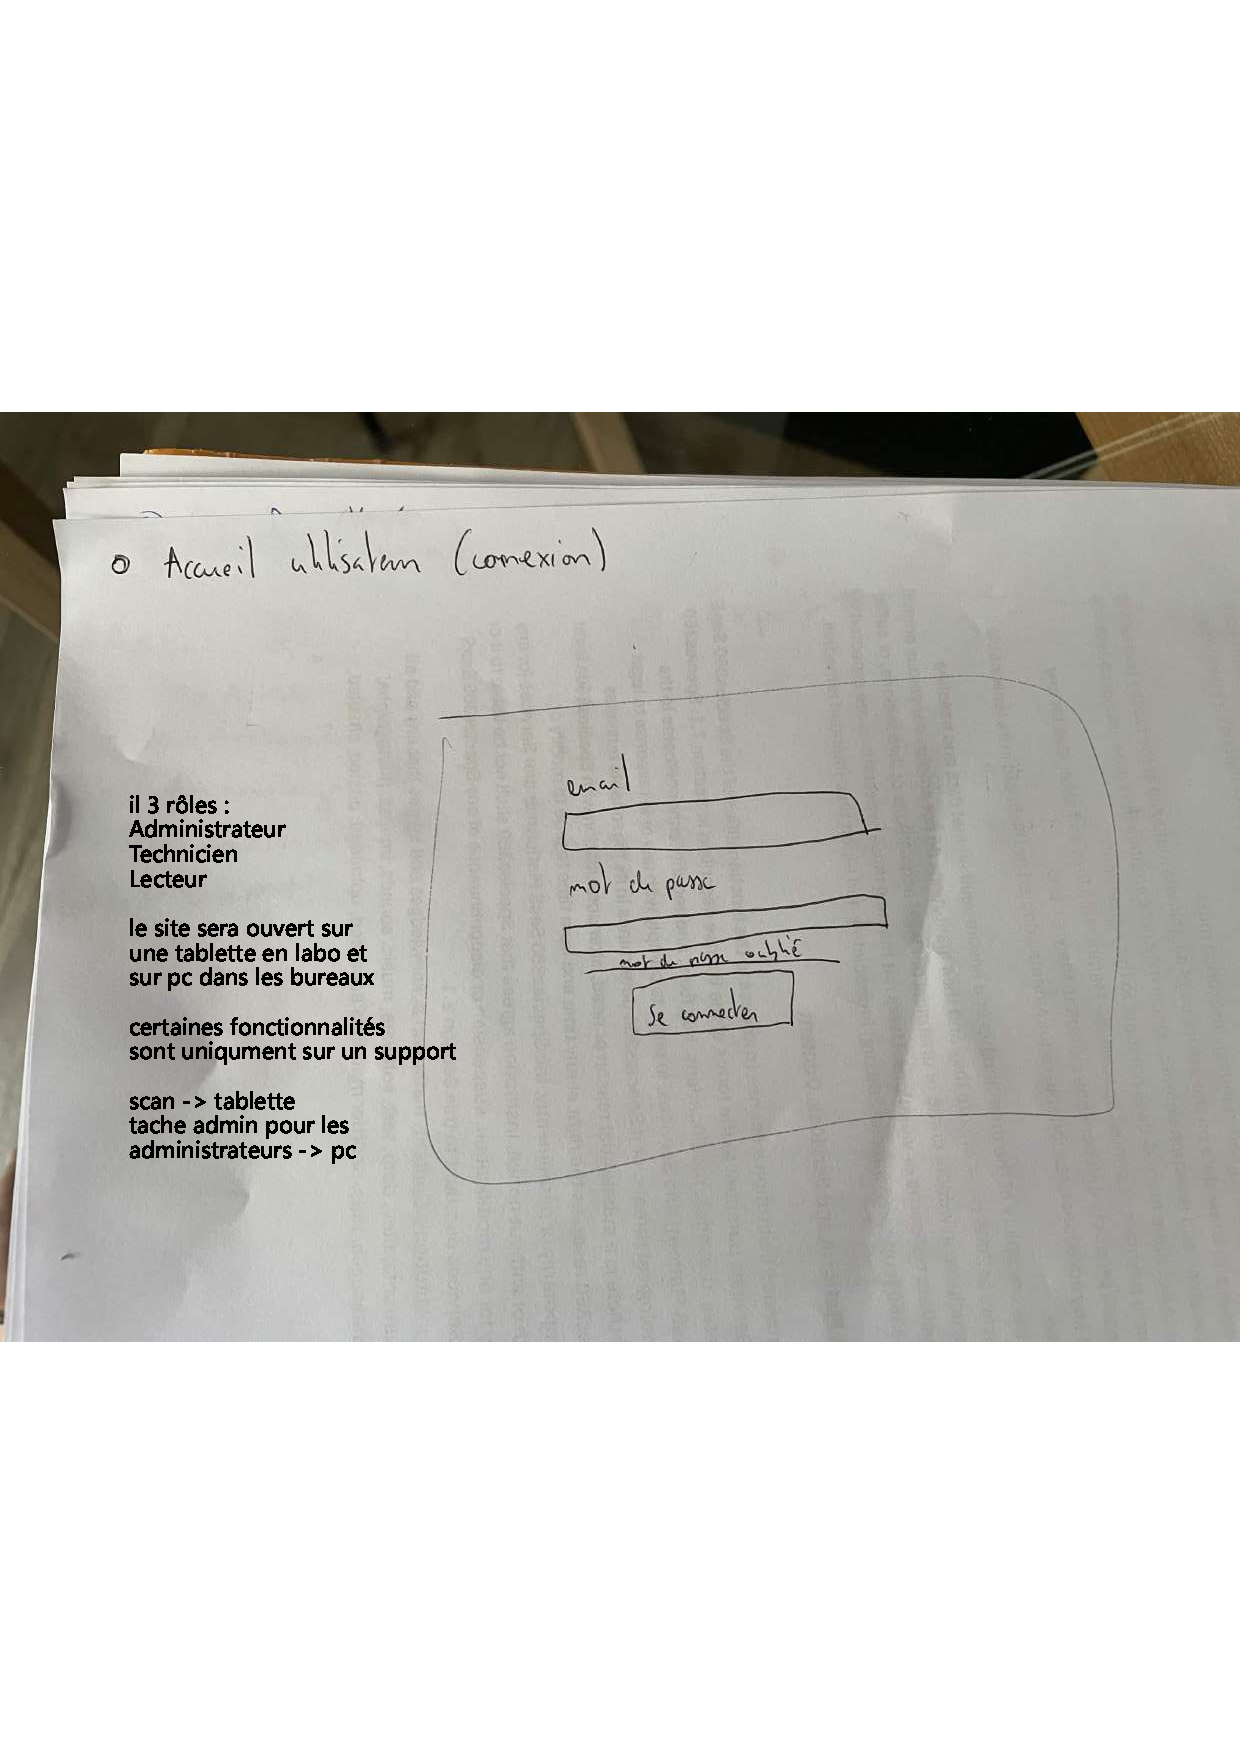
\includegraphics[page=1,width=0.78\textwidth]{docs/maquette_papier/maquette.pdf}
\caption{Extrait de la maquette papier utilisée pour cadrer les premiers écrans.}
\vspace{-0.35cm}
\caption*{\footnotesize Source : \texttt{docs/maquette\_papier/maquette.pdf}.}
\label{fig:maquette-papier}
\end{figure}

Le travail mené jusqu’à présent pose les bases de cet outil. Le projet contient une architecture Django et React, un modèle de données métier, une API avec Django REST Framework, des données de démonstration, une première interface, un système de traduction français anglais, une page de confidentialité et un notebook d’analyse exploratoire des anciens fichiers Excel. L’application reste en construction et transforme déjà un besoin de laboratoire en structure logicielle maintenable.

\section{État de l’art et cadrage}

Le projet s’inscrit dans plusieurs familles de références. La première est celle de la numérisation d’un suivi de laboratoire. L’objectif est de rendre les données plus traçables, de conserver leur historique, de retrouver rapidement une boîte et de préparer une réutilisation scientifique ou réglementaire des relevés.

La deuxième référence est celle des plateformes existantes pour aquariums. La référence la plus claire dans les notes de travail est Fauniabase, un logiciel de Luxaqua destiné à la gestion et au suivi des animaux dans les aquariums publics. Le service le présente comme un outil pour centraliser les données, suivre les poissons et les bacs, gérer la traçabilité, planifier des tâches et utiliser des QR codes.\footnote{\url{https://www.luxaqua.tech/fr/fauniabase/}} Cette référence montre qu’il existe déjà des outils professionnels autour de la gestion d’inventaires vivants en aquarium.

Fauniabase apporte une référence utile pour Polypbase. Polypbase cible toutefois un besoin plus spécialisé : les cultures de polypes de méduses, leurs relevés réguliers, leur historique, les repiquages, les conditions de température et l’usage en laboratoire sur tablette. Le travail retient surtout certaines idées utiles, comme la centralisation des données, la traçabilité, la recherche rapide et l’identification par QR code.

Une autre plateforme présentée pendant le cadrage a surtout servi de contre exemple. Elle rassemblait beaucoup d’informations avec un usage lourd, une navigation complexe, de nombreuses références et plusieurs termes pour désigner des objets proches. Ce type d’outil montre le risque principal pour Polypbase. Dans un laboratoire, l’utilisateur doit pouvoir saisir un relevé sans devoir comprendre une architecture compliquée. L’application doit utiliser des codes clairs, des écrans courts et des actions évidentes.

La troisième référence concerne la taxonomie. Une application utilisée par plusieurs structures doit éviter les ambiguïtés sur les noms d’espèces. Le World Register of Marine Species, ou WoRMS, répond à ce besoin en donnant accès à des noms valides, des synonymes, des noms vernaculaires et des identifiants stables pour les organismes marins.\footnote{\url{https://www.marinespecies.org/about.php}} Polypbase peut ainsi relier ses espèces à des références reconnues sans porter toute la complexité taxonomique. C’est pour cette raison que le modèle \texttt{Species} prévoit un identifiant WoRMS éventuel.

La quatrième référence vient de la biologie des méduses. Les articles sur les polypes et les éphyrules aident à justifier les données suivies. Helm rappelle que beaucoup de scyphozoaires ont un cycle comprenant une larve planula, un polype benthique et une méduse, et que la transformation du polype en éphyra s’appelle la strobilation.\footnote{\url{https://pubmed.ncbi.nlm.nih.gov/29446223/}} Fuchs et ses coauteurs montrent aussi que, chez Aurelia aurita, la transition du polype vers la méduse est déclenchée par des signaux environnementaux et que des protéines sont fortement activées avant la métamorphose en réponse aux changements saisonniers de température.\footnote{\url{https://doi.org/10.1016/j.cub.2013.12.003}}

La température apparaît donc comme une donnée importante à conserver. Une étude expérimentale sur trois espèces de scyphozoaires indique que la température peut jouer un rôle dans la reproduction asexuée des polypes, le moment de la strobilation et la production d’éphyras.\footnote{\url{https://doi.org/10.1016/j.jembe.2019.03.003}} Ces résultats expliquent l’intérêt de relier les comptages biologiques aux zones thermiques, aux sondes, aux changements de température et aux historiques de boîtes.

Le contexte scientifique de l’Aquarium donne aussi du sens au projet. Le LabCom Jellyfish and Polyps Academy explique que l’Aquarium de Paris maintient une grande collection de polypes de méduses et travaille avec MARBEC sur la culture des méduses, la création d’une banque de référence de polypes et la compréhension des paramètres qui influencent leurs proliférations.\footnote{\url{https://jellyfishandpolypsacademy.com/laboratoire/}} Polypbase s’inscrit dans cette logique. L’application doit aider à conserver des données plus propres, plus faciles à retrouver et plus adaptées à une analyse future.

\section{Analyse du besoin}

\subsection{Suivre des cultures de polypes}

Le coeur du projet est le suivi des boîtes de polypes. Dans le code, une boîte est représentée par le modèle \texttt{Box}. Elle appartient à une organisation, possède un code global, un code local, un numéro, une souche, une origine possible, une zone thermique et un statut. Cette structure permet de retrouver une boîte de manière unique, de la relier à une espèce et de suivre son emplacement.

Les relevés biologiques sont représentés par le modèle \texttt{BiologicalMeasurement}. Un relevé contient une date, un nombre de polypes, un nombre d’éphyrules, un nombre de strobiles, un état de culture, un indicateur d’attention, une note et un utilisateur. L’interface React actuelle se concentre sur les champs utiles à la saisie en laboratoire. Elle affiche les polypes, les éphyrules, le dernier commentaire, une zone d’observation et des boutons rapides pour ajouter des valeurs. Ce choix permet de simplifier la saisie sur tablette tout en gardant un modèle backend plus large.

Les observations sont séparées dans le modèle \texttt{Observation}. Elles permettent de stocker des commentaires plus qualitatifs, avec un type d’observation. Les notes de la maquette papier indiquent une observation facultative, une dernière observation toujours visible et un bouton discret pour afficher l’historique complet. La fiche boîte React suit cette logique en affichant le dernier commentaire au-dessus de la zone d’observation.

\subsection{Faciliter le travail en laboratoire}

La maquette papier indique que l’application sera utilisée sur tablette en laboratoire et sur ordinateur dans les bureaux. Sur tablette, l’objectif est de réduire les actions nécessaires. L’écran de pilotage met donc en avant la recherche ou le scan, les derniers accès et les suggestions de boîtes. La fiche boîte tablette regroupe l’identité de la boîte, le dernier relevé et l’accès à l’historique dans une zone compacte. La saisie du relevé du jour cache le champ de date sur tablette, car la date utilisée est celle du jour par défaut.

Le code React contient aussi des boutons d’incrémentation pour les valeurs. Les polypes peuvent être augmentés avec des boutons \texttt{+50} et \texttt{+100}. Les éphyrules peuvent être augmentées avec des boutons \texttt{+10} et \texttt{+25}. Cette logique répond à un besoin de saisie tactile rapide. Les valeurs pourront encore évoluer, car la maquette papier indique que les valeurs des boutons doivent être modifiées plus tard.

Le QR code est prévu dans le modèle avec \texttt{IdentificationTag}. Le modèle autorise des tags de type QR, NFC ou RFID, liés soit à une boîte, soit à une zone thermique. Les scripts contiennent aussi un fichier \texttt{generate\_qr\_codes.py}. Ce script contient pour l’instant un point d’entrée prévu pour une future génération de QR codes à partir des identifiants Django.

\subsection{Consulter les données sur ordinateur}

L’interface ordinateur doit rester plus confortable pour la consultation. Le code React contient trois onglets principaux dans l’état actuel : pilotage, zones et profil. La recherche donne accès aux boîtes et la fiche boîte affiche le dernier relevé, le formulaire et l’historique. Les zones thermiques affichent les températures, la salinité, les sondes et le nombre de boîtes. Le profil affiche l’utilisateur, ses organisations et le choix de langue.

Les exports et les vues liées aux boîtes font partie du périmètre prévu pour l’application principale. Le backend contient déjà le modèle \texttt{DataExport}, qui stocke le type d’export, le format, les filtres, le nom de fichier, l’utilisateur et la date d’export. Les vues d’export restent à développer.

\subsection{Gérer les rôles}

Le besoin distingue plusieurs rôles. La maquette papier mentionne trois rôles : administrateur, technicien et lecteur. Le modèle \texttt{OrganizationMembership} contient les rôles \texttt{admin}, \texttt{lab\_technician} et \texttt{viewer}. Les permissions du backend utilisent ces rôles pour limiter les actions de laboratoire. La fonction \texttt{user\_can\_write\_lab\_data} autorise la saisie aux super utilisateurs, aux administrateurs et aux techniciens laboratoire. L’API refuse la création d’un relevé biologique pour un utilisateur en lecture seule.

Cette séparation est importante pour la maintenance et pour la sécurité. Elle évite de donner les mêmes droits à tous les utilisateurs. Elle prépare aussi l’utilisation par plusieurs organisations, avec des accès filtrés par structure.

\section{Choix d’architecture}

\subsection{Une architecture hybride}

Le choix retenu est hybride. Django garde la base de données, les API, l’authentification, l’administration, les exports serveur et les pages liées à la confidentialité. React sert pour l’application principale, qui doit être plus fluide pour la tablette et plus agréable à utiliser sur ordinateur.

Ce choix est cohérent avec le besoin observé dans le projet. Django est adapté aux modèles de données, aux permissions, aux formulaires serveur, à l’admin et aux exports. React est mieux adapté aux écrans interactifs, à la recherche, aux suggestions, à la fiche boîte et aux adaptations entre tablette et ordinateur. Le projet évite ainsi de demander à Django de porter toute l’expérience tablette, tout en évitant de mettre toute la logique métier dans React.

La structure du projet suit cette séparation. Le dossier \texttt{backend} contient Django, ses apps, sa configuration et ses dépendances Python. Le dossier \texttt{frontend} contient l’application React avec Vite. Le dossier \texttt{docs} regroupe les documents de cadrage, les maquettes, les notes et les MCD. Le dossier \texttt{scripts} contient les scripts prévus pour des tâches ponctuelles comme l’import Excel et la génération de QR codes.

\subsection{Django côté backend}

Django est utilisé pour stocker les données, gérer les comptes, exposer les API et préparer les futures fonctions serveur. Le projet utilise Django 5.2.13 et Django REST Framework 3.16.1. Les dépendances Python sont gérées avec \texttt{uv}, avec \texttt{pyproject.toml} et \texttt{uv.lock}.

La configuration de base de données permet deux situations. En développement local, si aucune variable \texttt{POSTGRES\_DB} n’est définie, Django utilise SQLite avec \texttt{backend/db.sqlite3}. Si les variables PostgreSQL sont présentes, Django utilise PostgreSQL via \texttt{psycopg}. Cette organisation permet de travailler simplement en local tout en gardant une configuration possible pour une base PostgreSQL.

\subsection{React côté frontend}

React est utilisé pour construire l’interface principale. Le frontend utilise Vite, React 18.3.1 et TypeScript. Les appels HTTP sont centralisés dans \texttt{frontend/src/api/client.ts}. Ce fichier contient des fonctions \texttt{apiGet}, \texttt{apiPost} et \texttt{apiPatch}. Les requêtes utilisent les cookies de session Django et ajoutent le jeton CSRF pour les requêtes qui modifient les données.

L’interface est encore une première version. Elle contient un écran de pilotage, une fiche boîte, une vue des zones thermiques et un profil. Elle distingue le rendu tablette du rendu ordinateur par CSS. Cette distinction est importante, car la version tablette doit être plus directe et plus compacte, tandis que la version ordinateur doit rester adaptée à la consultation.

\subsection{Gestion des dépendances}

Le projet utilise \texttt{uv} pour l’environnement Python. Les commandes de travail principales sont \texttt{uv venv}, \texttt{uv sync}, \texttt{uv add} et \texttt{uv run}. Ce choix facilite la reprise du projet, car les dépendances Python sont déclarées dans \texttt{pyproject.toml} et verrouillées dans \texttt{uv.lock}. Une personne qui récupère le projet peut recréer l’environnement sans dépendre du nom local de l’environnement virtuel.

Le frontend conserve sa gestion classique avec \texttt{npm install}, \texttt{npm run dev} et \texttt{npm run build}. Les dépendances JavaScript sont séparées dans \texttt{frontend/package.json}.

\section{Modèle de données}

Le modèle de données est réparti dans plusieurs apps Django. Cette séparation rend le projet plus lisible et plus maintenable. Elle évite de concentrer tous les modèles dans une seule app générale. Chaque app correspond à un domaine fonctionnel.

Le MCD présenté dans ce mémoire doit être lu comme une version de travail. Il a déjà été discuté et optimisé avec l’aide de Madame Sandra Bringay, afin de mieux clarifier les entités et les relations importantes. Le schéma doit donc être refait proprement avant d’être considéré comme une version finale. La figure ci-dessous conserve l’état disponible au moment de la rédaction, car elle permet encore de comprendre la logique générale du modèle.

\begin{figure}[H]
\centering
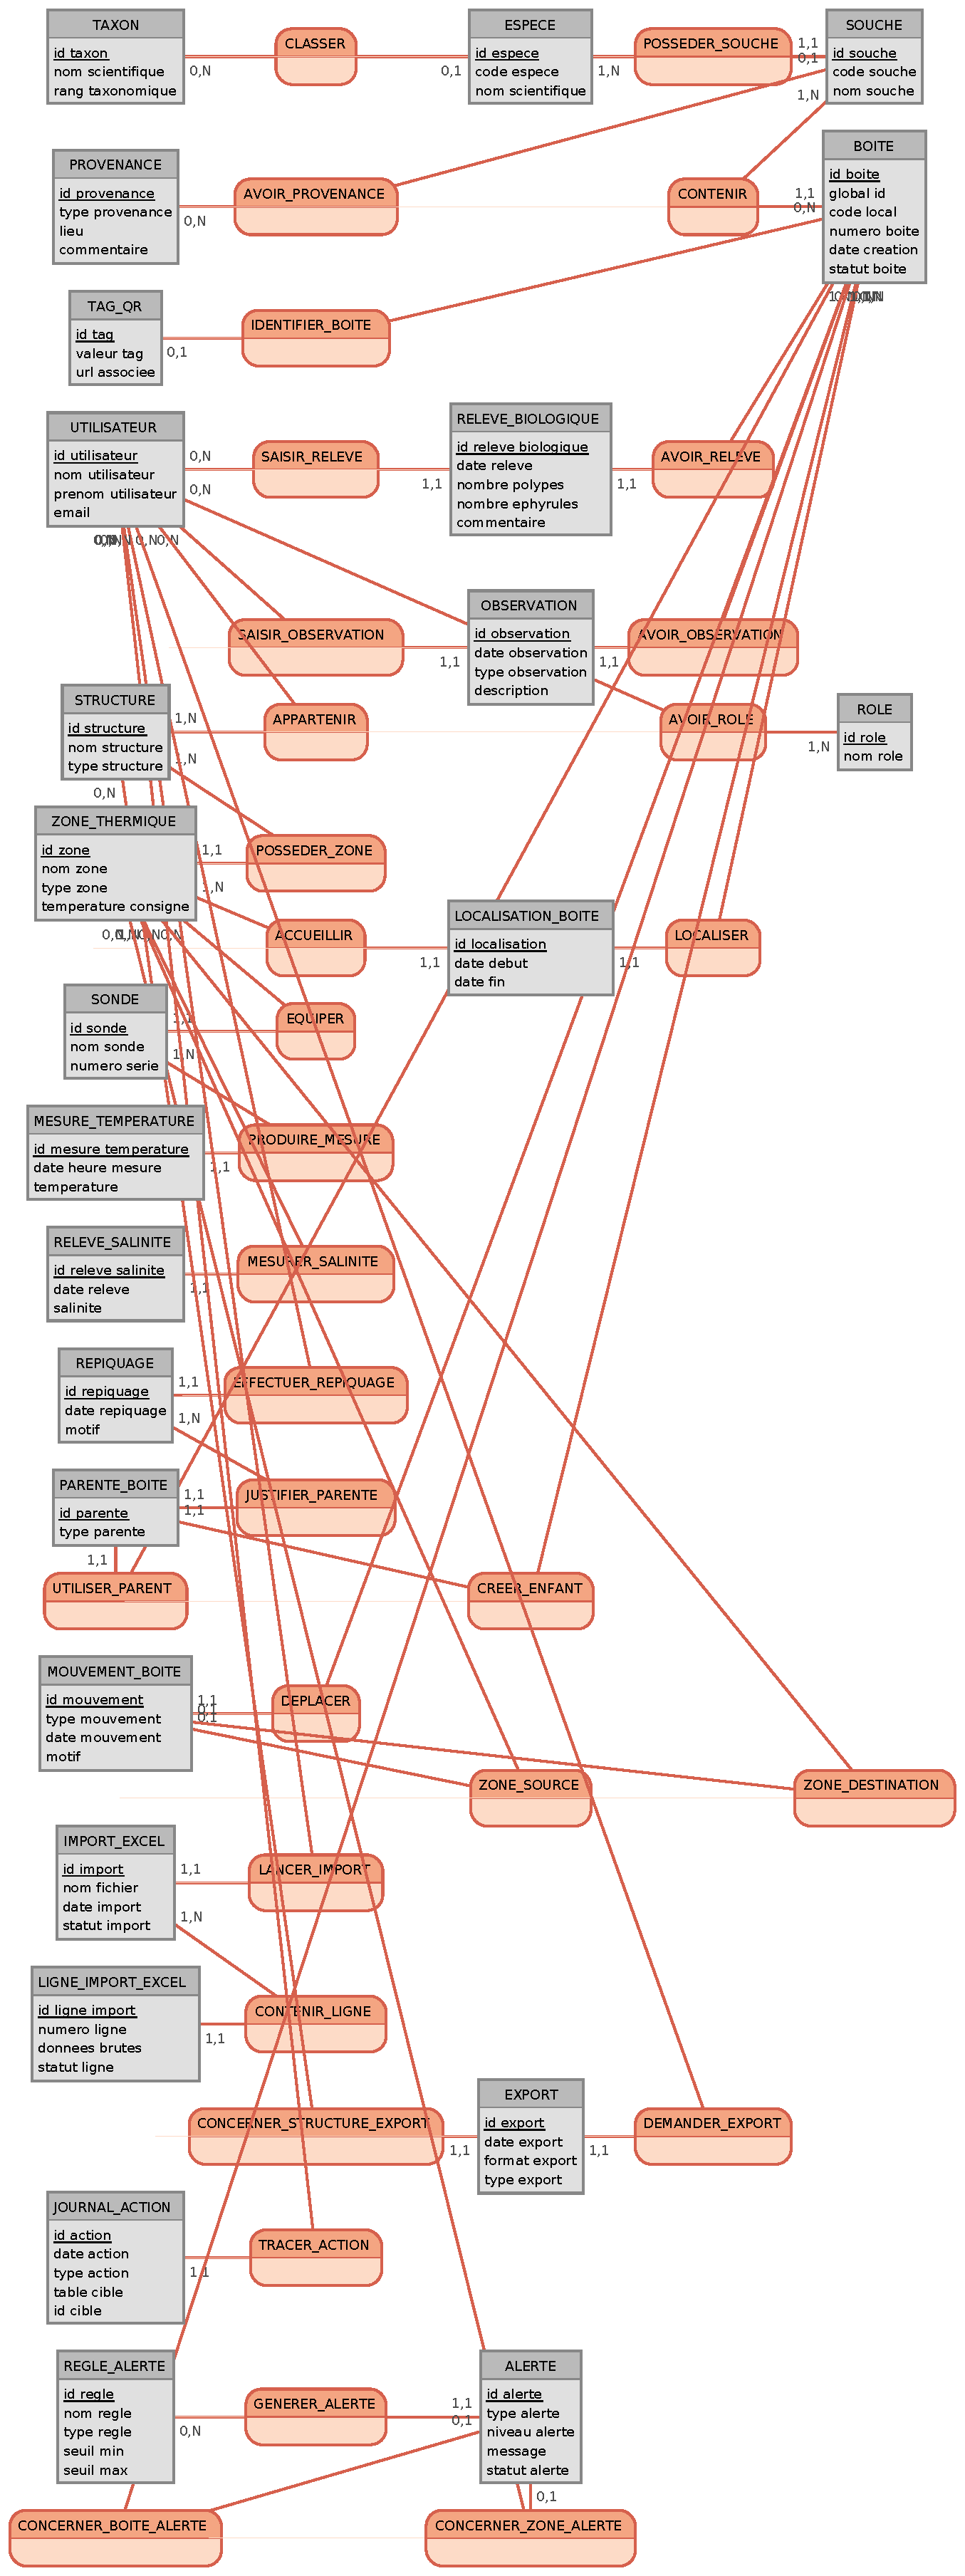
\includegraphics[height=0.78\textheight]{docs/mcd/MCD_complet.pdf}
\caption{Version de travail du modèle conceptuel de données Polypbase.}
\vspace{-0.35cm}
\caption*{\footnotesize Source : \texttt{docs/mcd/MCD\_complet.pdf}.}
\label{fig:mcd-complet}
\end{figure}

\subsection{Organisations et partenaires}

L’app \texttt{organizations} contient les structures qui utilisent ou partagent des données dans Polypbase. Le modèle \texttt{Organization} contient le nom, le slug, la ville, le pays, un email de contact, un statut actif et des notes. Le modèle \texttt{PartnerInstitution} permet de stocker une institution partenaire. Le modèle \texttt{SharingAgreement} décrit un accord de partage entre deux organisations, avec un statut et des droits séparés pour l’inventaire, les mesures et les exports.

Cette partie répond au besoin multi structure. Une boîte, une zone thermique, une sonde, une alerte ou un export est rattaché à une organisation. Les requêtes API filtrent ensuite les données selon les organisations autorisées pour l’utilisateur.

\subsection{Comptes et préférences}

L’app \texttt{accounts} gère les appartenances, les rôles et les préférences. Le modèle \texttt{OrganizationMembership} relie un utilisateur Django à une organisation avec un rôle. Le modèle \texttt{UserPreference} stocke la langue d’interface choisie par l’utilisateur. Les deux langues présentes sont le français et l’anglais.

Le middleware \texttt{UserInterfaceLanguageMiddleware} active la langue à chaque requête. Si l’utilisateur est connecté, la langue vient de sa préférence. Sinon, Django utilise la langue de session ou le français par défaut.

\subsection{Taxonomie}

L’app \texttt{taxonomy} décrit les espèces et les souches. Le modèle \texttt{Taxon} permet de construire une hiérarchie taxonomique. Le modèle \texttt{Species} contient le nom scientifique, le nom commun, le code espèce et un identifiant WoRMS éventuel. Le modèle \texttt{Origin} décrit l’origine d’une souche, avec un type de source, une date, une description, une institution, des coordonnées et des informations de collecte. Le modèle \texttt{Strain} relie une souche à une espèce et à une origine.

Cette organisation permet de relier une boîte à une souche, puis à une espèce et à une provenance. Elle prépare les filtres par espèce et par souche prévus pour la consultation et les exports.

\subsection{Cultures et boîtes}

L’app \texttt{cultures} regroupe les boîtes, les zones thermiques, les déplacements, les repiquages, la parenté, les tags et les transferts. Le modèle \texttt{ThermalZone} représente une armoire, une étuve, un bac ou une autre zone. Le modèle \texttt{Box} représente une boîte de culture. Le modèle \texttt{BoxLocation} conserve l’historique de localisation d’une boîte. Le modèle \texttt{BoxMovement} enregistre un mouvement entre zones.

Le repiquage est prévu avec \texttt{SubcultureEvent} et \texttt{BoxLineage}. Un repiquage crée un lien entre une boîte parent et une boîte enfant. Les notes de la maquette papier indiquent qu’un repiquage reprend la logique d’une nouvelle boîte avec des données préremplies, car un repiquage signifie créer un enfant qui hérite de certaines informations.

Le modèle \texttt{IdentificationTag} prépare l’identification par QR code, NFC ou RFID. Le modèle impose qu’un tag vise un seul objet, soit une boîte, soit une zone thermique. Le modèle \texttt{BoxTransfer} prépare les transferts de boîtes entre organisations.

\subsection{Mesures biologiques et environnementales}

L’app \texttt{measurements} contient les relevés biologiques, les observations, les sondes, les températures, la salinité et les anomalies thermiques. Cette séparation permet de distinguer les données biologiques saisies par le laboratoire et les données environnementales rattachées aux zones.

Le modèle \texttt{Probe} rattache une sonde à une zone thermique et à une organisation. Il prévoit plusieurs types, dont LoRaWAN, iMinilide, saisie manuelle et autre. Les modèles \texttt{TemperatureMeasurement} et \texttt{DailyTemperature} permettent de stocker des mesures ponctuelles et des agrégats journaliers. Le modèle \texttt{SalinityMeasurement} conserve les relevés de salinité. Le modèle \texttt{ThermalAnomaly} prépare la détection ou le stockage des anomalies.

\subsection{Exports et traçabilité}

L’app \texttt{exports} contient les imports Excel et les exports de données. \texttt{ExcelImport} décrit un import, \texttt{ExcelImportRow} stocke des lignes brutes et leurs erreurs éventuelles, et \texttt{DataExport} décrit un export avec son type, son format et ses filtres. La logique réelle d’import et d’export reste à relier aux scripts.

L’app \texttt{audit} contient les alertes et le journal d’action. \texttt{Alert} permet d’attacher une alerte à une boîte ou à une zone thermique. \texttt{AuditLog} conserve les actions importantes avec un utilisateur, une organisation, un type d’objet, une description et des métadonnées.

\section{API Django REST Framework}

L’API est exposée sous \texttt{/api/}. Les anciens endpoints prototypes en français, comme \texttt{/api/boites/} et \texttt{/api/zones/}, ont été supprimés. Les tests confirment que ces routes retournent une erreur 404. Le frontend doit utiliser les routes anglaises stables.

\begin{table}[H]
\centering
\small
\begin{tabularx}{\textwidth}{p{0.34\textwidth}Y}
\toprule
\textbf{Endpoint} & \textbf{Rôle} \\
\midrule
\texttt{GET /api/health/} & Vérifie que le service répond. Cette route est publique. \\
\texttt{GET /api/dashboard/} & Renvoie les données de synthèse pour le premier écran React. \\
\texttt{GET /api/boxes/} & Renvoie la liste paginée des boîtes, avec filtres par recherche, statut et organisation. \\
\texttt{GET /api/boxes/<id>/} & Renvoie le détail d’une boîte avec son historique de relevés. \\
\texttt{GET /api/boxes/<id>/measurements/} & Renvoie les relevés biologiques d’une boîte. \\
\texttt{POST /api/boxes/<id>/measurements/} & Crée ou met à jour le relevé d’une boîte pour une date donnée. \\
\texttt{GET /api/thermal-zones/} & Renvoie les zones thermiques, les sondes et les dernières mesures. \\
\texttt{GET /api/profile/} & Renvoie le profil utilisateur, ses organisations et sa langue. \\
\texttt{PATCH /api/profile/} & Met à jour les préférences du compte, dont la langue d’interface. \\
\bottomrule
\end{tabularx}
\caption{Endpoints API présents dans la configuration Django.}
\end{table}

Les permissions sont appliquées côté backend. La liste des boîtes utilise les organisations autorisées pour l’utilisateur. Le détail d’une boîte utilise le même filtrage. La création d’un relevé vérifie que l’utilisateur peut écrire des données de laboratoire. Si l’utilisateur n’a qu’un rôle de lecture, l’API refuse la création.

Le endpoint de création de relevé utilise \texttt{update\_or\_create}. Cela signifie qu’un relevé pour une même boîte et une même date est créé s’il n’existe pas, puis mis à jour s’il existe déjà. Une entrée de journal est ajoutée dans \texttt{AuditLog}. L’action est \texttt{ENTRY} lors d’une création et \texttt{UPDATE} lors d’une mise à jour.

Les tests backend couvrent les éléments principaux de cette première API. Ils vérifient que le endpoint de santé est public, que les anciennes routes françaises sont retirées, que la liste des boîtes est paginée et filtrée par organisation, que le détail renvoie l’historique des relevés, que la création de relevé fonctionne, que les utilisateurs en lecture seule sont bloqués, que les zones thermiques renvoient les sondes et les dernières mesures, et que le profil permet de modifier la langue.

\section{Interface React}

L’interface React actuelle est une première version fonctionnelle. Elle sert à tester le lien entre les données du backend et les écrans principaux attendus. Le code se trouve principalement dans \texttt{frontend/src/App.tsx}, avec les types dans \texttt{frontend/src/types.ts}, le client API dans \texttt{frontend/src/api/client.ts} et le style dans \texttt{frontend/src/styles/app.css}.

\subsection{Pilotage}

L’onglet pilotage sert de point d’entrée. Il propose une recherche par code, espèce ou souche. Il affiche aussi les derniers accès et des suggestions de boîtes. Lorsqu’une boîte est sélectionnée, l’application charge son détail via \texttt{/api/boxes/<id>/}. Cette logique permet d’aller rapidement vers la fiche d’une boîte sans passer par une liste longue.

Le code contient aussi une décoration visuelle avec de petites méduses en fond. Elle est placée dans le frontend public avec \texttt{frontend/public/jellyfish.svg}. Cet élément sert seulement à rendre l’interface moins froide, tout en gardant une faible présence visuelle.

\subsection{Fiche boîte}

La fiche boîte affiche le code global, l’espèce, le statut, la zone thermique, l’organisation, le dernier relevé, le formulaire de nouveau relevé et l’historique. Le formulaire envoie les données au backend avec \texttt{apiPost}, puis recharge la fiche pour afficher les informations à jour.

La version ordinateur conserve une présentation plus complète. La version tablette est séparée par CSS. Elle fusionne l’identité de la boîte et le dernier relevé dans une bande haute plus compacte. Sur tablette, le bouton \textit{Voir relevés} ouvre l’historique dans une fenêtre. Cette décision vient de l’objectif de simplification en laboratoire.

Sur tablette, le champ de date est caché pour éviter une saisie inutile dans le cas courant. La date par défaut vient de la date du jour. La date reste visible sur ordinateur, car l’usage de consultation et de correction est moins contraint par la taille de l’écran.

\subsection{Zones thermiques}

L’onglet zones affiche les zones thermiques accessibles à l’utilisateur. Les données viennent de \texttt{/api/thermal-zones/}. Chaque zone contient son organisation, sa température cible, son statut, le nombre de boîtes, la dernière température, la dernière salinité et les sondes associées.

Cette partie est importante pour relier les boîtes à leur environnement. Le cadrage a aussi mis en avant les températures hebdomadaires, les anomalies thermiques et les effets possibles sur les polypes. Le modèle actuel prépare cette relation entre zones, sondes, températures, salinité et boîtes.

\subsection{Profil et langue}

L’onglet profil affiche l’utilisateur connecté et ses organisations. Il permet aussi de changer la langue de l’interface entre français et anglais. Le français est la langue par défaut, car l’outil est d’abord utilisé par l’équipe de l’Aquarium de Paris. L’anglais est prévu pour permettre une utilisation par d’autres aquariums ou structures partenaires.

Côté backend, la préférence est stockée dans \texttt{UserPreference}. Côté React, la langue active est utilisée pour afficher les textes de l’interface. Côté Django, les fichiers de traduction se trouvent dans \texttt{backend/locale/fr/LC\_MESSAGES/django.po} et \texttt{backend/locale/en/LC\_MESSAGES/django.po}. Le projet contient aussi un script de compilation des traductions, car la commande Django officielle dépend de GNU gettext, parfois absent sur Windows.

\section{Analyse exploratoire des fichiers Excel}

Les fichiers de suivi historiques montrent comment les données sont réellement notées par l’équipe. Les fichiers \texttt{Suivi\_2019.xlsx} à \texttt{Suivi\_2026.xlsx} sont organisés par années. Dans ces fichiers, les feuilles correspondent à de grands groupes comme Aurelia, Hydrozoa, Cubozoa, Rhizostomae, Semaestomeae ou Coronatae. Certaines années ajoutent aussi d’autres feuilles, comme UMR\_MARBEC ou Staurozoa.

Dans les feuilles annuelles, les premières colonnes décrivent l’espèce, le numéro de boîte et la température. Les colonnes suivantes correspondent aux semaines ou aux mois de suivi. Pour une même boîte, les données sont notées sur plusieurs lignes, avec une ligne pour le nombre de polypes et une autre pour le nombre d’éphyrules. Cette forme facilite la saisie dans Excel semaine après semaine. Une base relationnelle demande une structure différente, avec une observation par ligne, une date, une boîte, un type de mesure et une valeur.

Le dossier de données contient aussi des fichiers complémentaires. Le fichier \texttt{ChangementT°C\_Repiquage.xlsx} regroupe un planning de repiquages et de changements de température. Le fichier \texttt{SuiviStrobilation.xlsx} contient des informations liées à la strobilation, avec des colonnes comme l’espèce, la température, la salinité et des conditions expérimentales. Le fichier \texttt{A.limbata.xlsx} reprend une structure plus déjà normalisée, avec une colonne de date et des groupes de colonnes associant une boîte, les polypes, les éphyrules et la température. Ces différences demandent un import plus fin qu’un simple copier coller. Il faudra reconnaître plusieurs formes de fichiers.

Deux fichiers CSV montrent déjà une transformation vers un format long. \texttt{polyp\_tracking\_long\_format.csv} utilise des noms de colonnes en anglais, comme \texttt{file\_year}, \texttt{group}, \texttt{species}, \texttt{box}, \texttt{temperature}, \texttt{measurement\_type}, \texttt{week\_index} et \texttt{value}. \texttt{suivi\_polypes\_format\_long.csv} contient le même principe avec des noms de colonnes en français. Cette structure est proche de ce dont Polypbase aura besoin pour alimenter les modèles Django.

Le notebook \texttt{notebooks/excel\_eda.ipynb} documente cette première analyse exploratoire. Son rôle est de comprendre la structure des fichiers, d’identifier les colonnes, de repérer les valeurs réellement saisies et de préparer une transformation utilisable par l’application. Il insiste aussi sur un point important. Une cellule vide peut avoir un sens différent de zéro. Elle peut correspondre à une absence de suivi, à une boîte inactive, à une période avant ou après un changement de température, ou à un repiquage qui a modifié le suivi. Un zéro saisi et une absence de valeur portent donc deux informations différentes.

L’import Excel réel reste à implémenter dans l’application. Le script \texttt{scripts/import\_excel.py} contient seulement un point d’entrée et un message indiquant que l’import reste à développer. La prochaine étape sera de transformer les règles observées dans les fichiers en code fiable. Il faudra aussi valider ces règles avec l’équipe de l’Aquarium, car certaines décisions demandent une confirmation métier.

\section{Intégration des sondes}

Le dossier \texttt{docs/sondes} contient une note d’intégration pour la sonde iMinilide-A. Cette note indique que l’appareil est un enregistreur autonome de températures Microlide, avec une connexion Ethernet RJ45. Elle indique aussi que la page web locale est accessible en HTTP sur le port 80 et renvoie des données XML. Cet accès local donne des valeurs en temps réel.

La même note décrit plusieurs modes d’accès. Le ModbusTCP, le logiciel iMinilog et le cloud Microlide dépendent d’une licence appelée Clé Soft. La page web locale et l’export USB sont indiqués comme disponibles sans licence. La note précise aussi que la sonde est sur le réseau local de l’aquarium. Un accès depuis l’extérieur demanderait un VPN ou une configuration réseau spéciale.

Le modèle Django est déjà préparé pour cette intégration. \texttt{Probe} contient un type \texttt{iminilide}. \texttt{TemperatureMeasurement} peut stocker les mesures ponctuelles, avec la source et les données brutes en JSON. \texttt{DailyTemperature} peut stocker des agrégats journaliers. \texttt{ThermalAnomaly} peut représenter des anomalies.

La logique d’intégration reste à écrire. La note indique que le format exact du XML devra être obtenu en inspectant la réponse réelle de la sonde physique. Le fichier \texttt{backend/apps/measurements/services.py} accueillera la logique d’interrogation, de parsing et de stockage.

\section{Confidentialité et sécurité}

Le projet contient une page \texttt{politique\_confidentialite.html}. Elle indique que Polypbase collecte les informations nécessaires au suivi des cultures, à la gestion des comptes et à la traçabilité scientifique des actions. Elle mentionne les données de compte, les données métier et les données de traçabilité.

La page explique aussi que les données servent à exécuter le service de suivi de collection, sécuriser l’accès, produire des exports et conserver l’historique du laboratoire. Elle indique que les utilisateurs peuvent demander l’accès, la rectification ou la suppression de leurs données de compte auprès de l’administrateur de leur organisation. Elle précise que les données scientifiques déjà liées à un historique de laboratoire peuvent être anonymisées si leur suppression compromet la traçabilité de la collection.

La sécurité actuelle repose d’abord sur les comptes Django, les sessions, les rôles et le filtrage par organisation. Django REST Framework utilise l’authentification par session et demande une authentification par défaut pour les routes API. Les requêtes React incluent les cookies et le jeton CSRF pour les actions d’écriture. En production, la page de confidentialité indique que l’application doit être servie en HTTPS, avec des sauvegardes régulières et une base de données non exposée directement aux terminaux du laboratoire.

\section{Travail réalisé à ce stade}

Le projet a avancé par étapes. Il a d’abord été initialisé avec Django. Les modèles métier ont ensuite été ajoutés, puis l’arborescence a été structurée en \texttt{backend}, \texttt{frontend}, \texttt{docs}, \texttt{scripts} et \texttt{notebooks}. Une première fiche boîte et un formulaire de relevé ont été créés, puis le backend a été refactorisé en apps Django séparées.

Une première API propre a été mise en place avec Django REST Framework. Les anciens endpoints prototypes en français ont été retirés. Les endpoints actuels sont vérifiés par des tests. Le formulaire de relevé React a ensuite été connecté à l’API. Le projet contient aussi une commande \texttt{seed\_demo\_data} qui crée un jeu de données local de démonstration. Cette commande crée des utilisateurs, des organisations, des souches, des zones, des sondes, des boîtes, des relevés, des observations, des alertes, de la parenté, des transferts, des imports et des exports de démonstration.

Le système de traduction a été ajouté. Le français est la langue par défaut et l’anglais est prévu comme seconde langue. La préférence est modifiable dans le profil. Le projet contient les fichiers \texttt{.po} et \texttt{.mo}, ainsi qu’un script de compilation compatible avec l’environnement Windows du projet.

Le frontend React contient une première interface. Elle permet de rechercher une boîte, d’afficher une fiche, de saisir un relevé, de consulter les zones thermiques et de modifier la langue dans le profil. La version tablette a été adaptée séparément de la version ordinateur afin de répondre au besoin de saisie en laboratoire. Le style reste volontairement épuré, avec peu d’informations visibles en même temps sur tablette.

Le projet a aussi été préparé pour une meilleure reprise par d’autres développeurs. La structure, les commandes, les apps cibles, les endpoints, les langues et les règles de commentaires sont documentés. Les dépendances Python sont gérées avec \texttt{uv}. Les données réelles sont exclues du versionnement avec \texttt{/data/} dans \texttt{.gitignore}. Les scripts d’import Excel et de QR code indiquent clairement les implémentations restantes.

\section{Ce qui reste à faire}

La première suite logique concerne l’import Excel. Le notebook montre qu’une transformation en format long est possible. Le script d’import réel reste à écrire. Il faudra définir précisément les correspondances entre les colonnes Excel et les modèles Django. Il faudra aussi valider le sens des cellules vides, des changements de température, des repiquages, des groupes et des feuilles complémentaires.

La deuxième suite concerne les QR codes. Le modèle \texttt{IdentificationTag} et le script \texttt{generate\_qr\_codes.py} montrent que le besoin est prévu. La génération reste à implémenter. Il faudra décider où stocker les QR codes générés, comment les imprimer et comment garantir que le code renvoie vers la bonne boîte ou la bonne zone.

La troisième suite concerne les exports. Le modèle \texttt{DataExport} peut déjà stocker un type d’export, un format et des filtres. Il faut encore construire les vues et les services qui produisent réellement les fichiers CSV ou XLSX. Les filtres devront permettre de sélectionner des espèces, des souches, des zones et des périodes.

La quatrième suite concerne les sondes. Les modèles sont prêts. Le service d’intégration reste à écrire. La note iMinilide indique qu’il faut relever l’adresse IP, inspecter le XML brut, identifier les voies et vérifier la présence d’une Clé Soft. La finalisation du parser dépend de ces informations.

La cinquième suite concerne l’interface d’administration métier. Django fournit déjà une administration technique. Les écrans React doivent encore couvrir la gestion prévue. Les notes indiquent que les tâches d’administration sont surtout prévues sur ordinateur. Il faudra donc ajouter des écrans pour les utilisateurs, les organisations, les zones, les sondes, les exports, les imports et les règles de partage.

La sixième suite concerne les tests en situation réelle. Le projet contient déjà des tests backend. L’interface tablette doit encore être testée sur le format matériel visé. Les maquettes indiquent une utilisation en laboratoire sur tablette. Il faudra vérifier la lisibilité, la taille des boutons, la navigation, la saisie tactile et le comportement en orientation paysage.

\section{Conclusion}

Polypbase est déjà passé du simple cadrage à une base technique exploitable. Le projet contient une architecture hybride claire, un backend Django structuré, une API propre, des modèles métier cohérents, une première interface React, une gestion des langues, une page de confidentialité, des données de démonstration et un notebook d’analyse exploratoire des fichiers Excel.

Le travail réalisé pose les fondations d’une application encore en construction. Les choix faits vont dans le sens d’un outil maintenable : les domaines métier sont séparés en apps Django, l’API utilise Django REST Framework, React est réservé à l’interface principale, les dépendances Python sont gérées avec \texttt{uv} et les données réelles restent hors du versionnement.

La suite doit transformer ces fondations en outil complet. Les points les plus importants sont l’import réel des fichiers Excel, la génération des QR codes, les exports filtrés, l’intégration des sondes et l’enrichissement des écrans d’administration. Ces étapes devront garder la même exigence de prudence : éviter les déductions fragiles, valider les règles métier avec l’Aquarium et conserver un code suffisamment clair pour être repris après le stage.

\end{document}
